\section{Self-organizing recurrent neural network (SORN)}
\label{sec:nn}

\subsection{Artificial neural networks}
\label{sec:ann}

Two different scientific approaches motivate an \acfi{ann}. Originally those networks were invented to simulate processes in the brain to get a better understanding of how the brain stores and processes information and how recognition and behavior is influenced by neural activity. Especially \textcite{rosenblatt1958perceptron} formulated a first idea to simulate a simple neural system, the so called \emph{perceptron}. On the other side, the idea came up to construct classification and prediction algorithms using \acs{ann}. Even though the approach was promising, for a long time artificial networks were not useful, because networks are computational costly and need big datasets to perform well. But when \textcite{hinton2006fast} published a fast way to train \acs{ann} and computers became more powerful at the same time, \acs{ann} became a widely used approach in machine learning. In machine learning \emph{supervised} \acs{ann}, where the algorithms learns with a given `truth', are still inspired by biology, but in most cases very different from real neural networks. On the other hand, computational neuroscience uses mostly \emph{unsupervised} networks, since there is no evidence that humans learn from an absolute truth. Those networks mostly try to be as close as possible to real neural processes or try to understand specific properties of biological networks. Nevertheless, in computational neuroscience the used networks highly depend on the level of research. For research on cell level, many details of neural conduction and synapses behaviors are modeled. Otherwise, if models on higher levels with hundreds or thousands of neurons are build, e.g. modeling memory and learning, many biological details on cell level are omitted in order to reduce complexity.

Independent of the approach, the basic principle for modeling neurons is the perceptron. Statistically the perceptron can be understood as a \ac{glm}, classifying the incoming signals either directly as $0$ or $1$ or giving a probability for those classes.

Beginning with a regression model, some inputs $\bm x \in \R^d$ are chosen to describe some output $y \in \R$, using a \emph{regression function} $f(\bm x)$. The regression is of the form

\begin{equation}
y = f(\bm x) + \epsilon.
\label{eq:gen-reg}
\end{equation}

Instead of the direct data $\bm x$ it is also possible to use a transformation $\phi(\bm x)$, which is called a \emph{feature}. For modeling a neural network, data $\bm x$ is used directly. $\epsilon \in \R$ is a stochastic error term, a random variable, and can be distributed in several ways. In most applications it is assumed to be normally i.i.d. distributed with $\epsilon \sim N(0,1)$. The regression function $f(\bm x)$ can be arbitrary. In a linear case it has the form

\begin{equation}
f(\bm x) = \bm x^T \bm \beta,
\end{equation}

where $\bm \beta \in \R^d$ are the parameters of dimension $d$. While the estimator of a linear model is relatively easy to obtain, an estimator for a non-linear $f(\bm x)$ is not easy to find. In order to have the opportunity to use non-linear models, in \ac{glm}s a so called link function $g^{-1}(f(\bm x)) = g^{-1}(\bm x^T \bm \beta)$ is introduced. It brings non-linearity to a linear model. If the expected value of $y$, modeled with the link function, is taken, it results in

\begin{equation}
\mu = \E[y] = \E[g^{-1}(\bm x^T \bm \beta) + \epsilon] = g^{-1}(\bm x^T \bm \beta),
\end{equation}

since $g^{-1}(\bm x^T \bm \beta)$ is deterministic and $\E[\epsilon] = 0$. At that point, the derived statistical model can be mapped to an \acs{ann} use case. $\bm x$ can be identified with the input signals from all pre-synaptic neurons $\bm z$ from equation \eqref{eq:activation}, where the first input is a dummy and is set to one. Furthermore, it can be seen that $\bm\beta$ is equal to the weights $\bm w_i$, where the first weight is $-b_i$. It means that $\sum_{j=1}^{n_i} w_{ij} z_j - b_i = \bm x_j^T \bm\beta_j$. Finally, the inverse of the link function $g^{-1} = \sigma$ is the \emph{activation function}, introduced in section \ref{sec:inhib-excit}, and $o = \mu$ denotes the output at the post-synaptic neuron. The output is given by

\begin{equation}
\label{eq:ann-model}
\mu = g^{-1}(\bm x^T \bm \beta) = g^{-1}\left(\sum_{j=1}^{n_i} w_{ij} z_j - b_i\right) \overset{\eqref{eq:activation}}{=} \sigma(a_i) = o.
\end{equation}

As already discussed in section \ref{sec:inhib-excit}, the choice of the activation function depends on the requirement. In machine learning, classically, a continuous function like a sigmoid or, more recent, piecewise rectified linear units (ReLUs) are used, since derivations are often necessary. In that case, there is always some activation, which rises strongly, if the input neurons increase in activity. Statistically, the perceptron with a sigmoid function is a logistic regression. 
 
In case of an indicator function, an all-or-none law is realized, which is a closer approximation to real neurons. It results in zero activity, if the input neurons sum to a value below the threshold and an activity of one, if the sum of the activity hits the threshold. Such an indicator function was introduced in equation \eqref{eq:heavi}.

So far, the perceptron model is able to simulate some pre-synaptic neurons and one post-synaptic neuron, which depends on the activity of the pre-synaptic neurons and the activation function. If multiple perceptrons are modeled, the output of one neuron can be an input for another neuron and so forth. Mathematically, a neural network with multiple neurons is a recursive \acl{glm}. It can be modeled in one direction with a \emph{feed forward} structure or in arbitrary directions with a \emph{recurrent} structure.

\subsection{Classification of ANN}

Over time, a large number of network types were developed. Besides many different architectural types, two important types will be mentioned here:

\begin{itemize}
\item \emph{Feed-forward neural networks} are basically multilayer perceptrons, where synapses are just built in one direction. The flow of information is going from input neurons to output neurons with hidden layers inbetween.
\item \ACFI{rnn} have neurons which have synapses not only reaching into the next layer, but also to a neuron in next time step of processing. Therefore, time-coded information can be included.
\end{itemize}

Another possible classification refers to the number of connections. A \emph{fully connected} network has all connections established, and therefore weights of non-zero between all neurons. A \emph{sparsely connected} network has just some few connections, whereas most connections are fixed to zero. In some networks, like Echo State Networks (see below), the connectivity is in an order of about $1\%$.

\subsection{Reservoir Networks}
\label{sec:res-net}

A specific case of \acs{rnn} is \emph{Reservoir Computing} \parencite{lukovsevivcius2009reservoir}. Those networks can be called reservoir networks. Input signals are fed into a sparsely and randomly connected network, called \emph{reservoir}. The reservoir behaves like a complex nonlinear dynamic filter that transforms the incoming signals using a high-dimensional temporal mapping \parencite{schrauwen2007overview}. Schrauwen et al. described similarities between reservoir computing and kernel methods. Kernel methods are often used in machine learning to transform the input into a multi-dimensional or even infinite-dimensional feature space, where linear separation or linear fitting performs better than in the original input space. Similar to kernels, also a reservoir can be seen as a transformation of the input into higher dimensions, where the readout is kind of a feature space. If the reservoir contains $N$ neurons, the input is projected into a $N$-dimensional space. A state of the reservoir is mathematically just a point in this high dimensional space. Temporal signals entering the reservoir can be described as a trajectory in that space. \textcite{lazarphd2009self} hypothesized in her dissertation that, theoretically, the brain computes with trajectories in a similar way, which would justify the use of reservoir networks in neural computation approaches.

Two major types of Reservoir Networks are \ac{esn} \parencite{jaeger2004harnessing} and \ac{lsm} \parencite{maass2002real}. Both networks were independently developed \parencite{goodfellow2007deep} and are quite similar. \ac{lsm} uses neurons with binary outputs. They are designed to explain processes in the brain, whereas \ac{esn} uses continuous hidden units and focuses on machine learning tasks. Under the condition of the \emph{separation property} (different inputs result in separable outputs) and the \emph{fading memory property} (information about recent input can be maintained) the \ac{lsm} fulfills the Stone-Weierstrass theorem, namely that the \ac{lsm} can approximate any continuous function \parencite{maass2004computational}. Therefore \ac{lsm} is an interesting starting point for reservoir based neural simulation.

\subsection{Self-organizing recurrent neural network (SORN)}
\label{sec:sorn}

\ac{lsm} are developed for supervised learning and parameters are trained in a way to minimize the error. To simulate brain dynamics it is necessary to find a more unsupervised way of learning. Furthermore, those networks have normally a static reservoir, which means that the weights are randomly initialized and fixed in further processing. To tackle both problems, plasticity rules are a promising approach. They could be used as described in section \ref{sec:plasticity}. There were already some additions to \acl{lsm}, like adding hebbian learning \parencite{norton2006preparing}, but a first sophisticated reservoir network with plasticity was proposed by \textcite{lazar2009sorn}, called a \acfi{sorn}. It uses three plasticity rules in a reservoir network with binary threshold neurons, namely:

\begin{itemize}
\item \ACF{stdp}
\item \ACF{sn}
\item \ACF{ip}
\end{itemize}

\paragraph{Plasticity rules}

\begin{wrapfigure}{R}{0.45\textwidth}
	\centering
	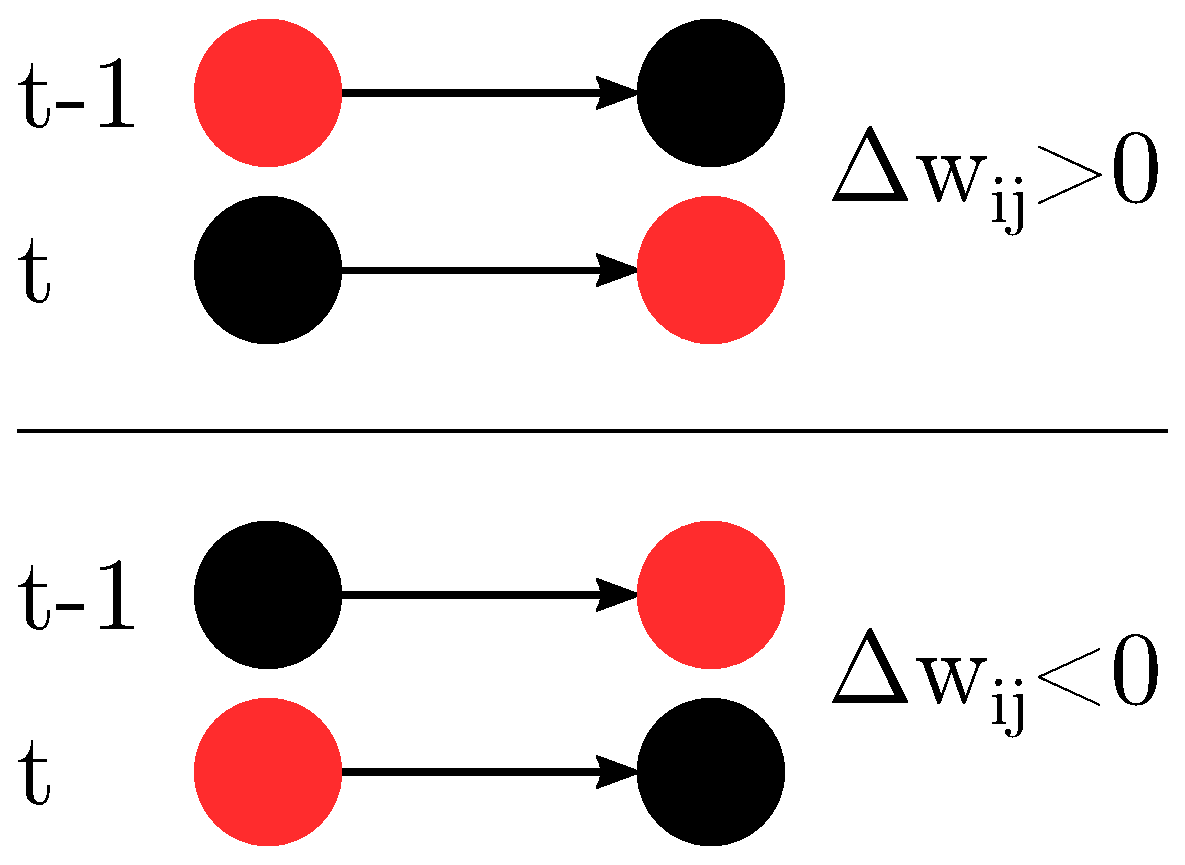
\includegraphics[width=0.45\textwidth]{sorn_markov/stdp}
    \caption[Spike-timing-dependent plasticity rule used in \acs{sorn}.]{Spike-timing-dependent plasticity rule used in \acs{sorn}. The black circle corresponds to a silent neuron, the red circle represents a spiking neuron. The arrow indicates the direction of the weight. If the pre-synaptic neuron is firing, before the post-synaptic neuron fires, the weight between them is increased. Otherwise, the weight is decreased.}
    \label{fig:stdp-simple}
\end{wrapfigure}

The \acl{sn} and \acl{ip} are realized according to equation \eqref{eq:sn} and equation \eqref{eq:ip} respectively. Regarding the \acs{ip}, recall that it is the source for spontaneous activity. \acs{sorn} is build such that noise is optional and in most applications the network is using spontaneous activity from \acs{ip} only. In consequence the system can be described as deterministic chaos, if the initial weights are given. Only if noise is included, it would truly behave stochastically. The only remaining stochastic part is the random initialization of the weights.

The \acl{stdp} can be derived from equation \eqref{eq:stdp-orig}. In \acs{sorn} only the last step in time and thus only one spike is considered. If the pre-synaptic neuron fires directly before the post-synaptic neuron, the weight is increased. Otherwise, the weight is decreased, as shown in figure \ref{fig:stdp-simple}. Hence, there is no summing necessary and the rule is simplified to

\begin{equation}
\Delta w_{ij}(t) = f(\Delta t) = f(t_j - t_i),
\end{equation}

where $t_j$ is the time when the pre-synaptic neuron $j$ spikes and $t_i$ when the post-synaptic neuron $i$ spikes. The learning window is defined as

\begin{equation}
f(\Delta t)
= \eta_\STDP \cdot \begin{cases} x_j(t_i - 1) x_i(t_i) & t_j \le t_i\\ -x_j(t_j) x_i(t_j - 1) & t_j > t_i \end{cases},
\end{equation}

\nomenclature{$\eta_\STDP$}{Learning rate for \acl{stdp}}

where the learning rate $\eta_\STDP$ was introduced. Note that $f(\Delta t)$ is zero, if both neurons are not active in a row. If $t$ denotes the absolute time of the network, the weight change can be simplified to

\begin{equation}
\label{eq:stdp}
\Delta w_{ij}(t) = \eta_\STDP \cdot \left( x_j(t-1) x_i(t) - x_j(t) x_i(t-1) \right),
\end{equation}

since $x_i(t), x_j(t) \in \{0,1\}$. Equation \eqref{eq:stdp} corresponds to \textcite[equation 5]{lazar2009sorn}.

What kind of plasticity rule is used, depends on the phase of training and testing. All the rules, which are included in a phase are applied after every discrete calculation step.

\paragraph{Network setup}

\nomenclature{$N^E$}{Number of excitatory neurons}
\nomenclature{$N^I$}{Number of inhibitory neurons}

\nomenclature{$W$}{Weight matrix}

\begin{figure}[t]
	\centering
	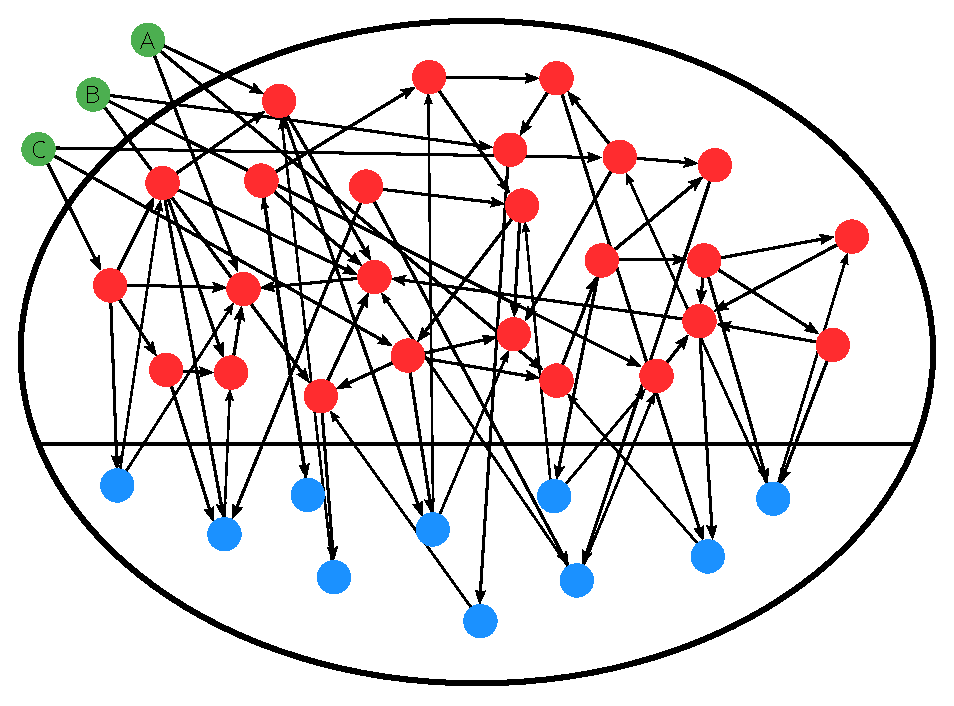
\includegraphics[width=0.6\textwidth]{sorn_markov/sorn}
	\caption[Sketch of the \acl{sorn}]{Sketch of the \acl{sorn}. Red circles are excitatory neurons, blue circles represent inhibitory neurons. Connections between excitatory neurons are sparse, inhibitory and excitatory neurons are fully connected in both directions. Input neurons are represented by green circles. They are connected to excitatory neurons.}
	\label{fig:sorn}
\end{figure}

$N^U$ is the number of input neurons and $N^E$ the number of excitatory neurons. Excitatory and inhibitory neurons were separated. The number of inhibitory neurons is set as a fraction of excitatory neurons, for example $N^I = 0.2 \cdot N^E$. All neurons have a weight of $w_{ij} \in [0,1]$. Weights are established between excitatory and excitatory neurons, modeled in a matrix $W^{EE}$, between inhibitory and excitatory neurons $W^{EI}$, excitatory and inhibitory neurons $W^{IE}$ and input neurons and excitatory neurons $W^{EU}$. The matrices $W^{EI}$ and $W^{IE}$ are fully connected, $W^{EE}$ is sparsely connected.

There are no connections between inhibitory and inhibitory neurons in the model. While those connections exist in real biological networks, they occur sparsely and their function is highly specialized \parencite{chamberland2012inhibitory}. Important are connections between excitatory and inhibitory neurons and vice versa. Those connections provide feedback loops, which help to stabilize the system \parencite{turrigiano2004homeostatic}. Finally, the target rate for the \ac{ip} was chosen as $H_{\text{IP}} = 2 \cdot N^U/N^E$.

The structure of the network is sketched in figure \ref{fig:sorn}.

\paragraph{Updating the network}

The general model, defined in equation \eqref{eq:ann-model}, can be specified for the  case of a \acs{sorn} network. $\bm x(t) \in \{0,1\}^{N^E}$ denotes the spiking state of the excitatory neurons and $\bm v(t) \in \{0,1\}^{N^U}$ represents the input neurons. In the next step of time, the state of the excitatory neurons is given by

\begin{equation}
\label{eq:update-excitatory}
x_i(t+1) = \Theta\left( \sum_{j=1}^{N^E} W_{ij}^{EE}(t) x_j(t) - \sum_{k=1}^{N^I} W_{ik}^{EI} y_k(t) + v_i(t) - T_i^E(t)\right).
\end{equation}

Note that $v_i(t) = \sum_{l=1}^{N^U} W_{il}^{EU} v_l(t)$. But since every excitatory neuron has not more than one connection to an input neuron, the notation is simplified by $v_i(t) \in \{0,1\}$. The threshold $T_i^E(t)$ depends on \acl{ip}, which was defined in equation \eqref{eq:ip}.

\nomenclature{$\bm x(t)$}{Spiking vector of excitatory neurons}
\nomenclature{$\bm y(t)$}{Spiking vector of inhibitory neurons}
\nomenclature{$\bm v(t)$}{Spiking vector of input neurons}

$\bm y(t) \in \{0,1\}^{N^I}$ denotes the spiking state of the inhibitory neurons. They are updated in a more simple way, using

\begin{equation}
\label{eq:update-inhibitory}
y_i(t+1) = \Theta\left( \sum_{j=1}^{N^E} W_{ij}^{IE} x_j(t) - T_i^I\right).
\end{equation}

The threshold $T_i^I$ for the inhibitory neurons is not updated using \acs{ip}. Also note that \acs{stdp} is applied to $W_{ij}^{EE}(t)$, but not to the inhibitory-to-excitatory weights, neither to the excitatory-to-inhibitory weights. $W_{ik}^{EI}$ and $W_{ik}^{IE}$ are not time-dependent. Consequently, also \acl{sn} is only applied to $W_{ij}^{EE}(t)$.

If input is given to the network, the network is trained. Without input, meaning that $v_i(t) = 0$ for all $i \in \{1, ..., N^E\}$, the network is left alone with spontaneous activity only. The presented equations can also be found in \textcite{lazar2009sorn}, where most of the notation is very similar. Further details regarding the readout and the training are also given in section \ref{sec:methods}.

\subsection{Properties of SORN}
\label{sec:prop-sorn}

Since \acs{sorn} was invented in 2009, many studies were done with this network. Results from four papers will be introduced, which show the performance of the network on one hand and the implications regarding the general understanding of dynamic biological networks on the other hand.

In the original paper from \textcite{lazar2009sorn}, the \acs{sorn} network was able to outperform static reservoir networks in several tasks. The network was tested in an `counting' and an `occluder' task. They were able to show that in both cases the performance of the \acs{sorn} was better than in networks where the weights were just initially set. \textcite{lazar2009sorn} argues that especially \ac{stdp} has an important role. There is a lot evidence that \ac{stdp}-like mechanisms are essential for stimuli encoding in the brain. In several experiments it was possible to show that repetitive stimulation with temporal patterned inputs causes a rapid reorganization, which bases on \ac{stdp} mechanisms \parencite{yao2001stimulus, fu2002temporal, yao2007rapid}.

\textcite{zheng2013network} extended the \ac{sorn} by two more plasticity rules. First, \emph{structural plasticity} was added in order to allow new synaptic connections between excitatory neurons. With a probability of $p_c = 0.1$ a new connection was established between a random pair of neurons with a weight of $w_{ij} = 0.001$. Since \ac{stdp} tends to silence some specific connections to a weight close to zero, the structural plasticity enabled the network to balance this effect. Second, \acfi{istdp} added \ac{stdp} from inhibitory to excitatory neurons. With this adapted \ac{sorn} network, it was possible to reproduce experimental findings from \textcite{yasumatsu2008principles}. The distribution of synaptic weight strengths in the \ac{sorn} matched the lognormal distribution of EPSPs in the visual cortex of rats.

An extension to a \acs{sorn} network is a \acfi{rmsorn}, which modulates the weight-changes in \ac{stdp} \parencite{aswolinskiy2015rm}. Equation \eqref{eq:stdp} gets an additional \emph{modulation factor} $m$, therefore
%
\begin{equation}
\label{eq:stdp-modulated}
\Delta w_{ij}(t) = m \cdot \eta_\STDP \cdot \left( x_j(t-1) x_i(t) - x_j(t) x_i(t-1) \right).
\end{equation}

Different modulation strategies can be used. The weight-change can be applied as normal, suppressed or inversed, depending on a favored output or readout. Within eight tasks \textcite{aswolinskiy2015rm} could show that \acs{rmsorn} is close to the performance of the original \ac{sorn} from \textcite{lazar2009sorn}, even though the \acs{rmsorn} learns more self-organized than the \ac{sorn}. It shows the ability of the \ac{sorn} network to learn even more complex tasks very well in a highly self-organized way.

Another huge research effort was done by \textcite{hartmann2015s}. First, they were showing that \ac{sorn} has many characteristics which can be observed in experimental findings. The following list contains four such findings, where the experimental studies are cited in brackets.

\begin{itemize}
\item The inter-spike-interval (ISI) distribution of a neuron can be fitted by an exponential decay. Furthermore, the coefficient of variation (CV) follows a Poisson distribution with an event rate around $1$ \parencite{kenet2003spontaneously, goris2014partitioning}.
\item The fraction of excitatory-to-excitatory connections, where the weight stays $w_{ij} > 0$ during plasticity, converges to a stable fraction \parencite{yasumatsu2008principles}.
\item Sequences of four distinct activity patterns can be learned. In the original experiment with mice, gratings were used to train the visual cortex V1 \parencite{gavornik2014learned}.
\item Those sequences can be predicted, using the stored information of the network \parencite{gavornik2014learned}.
\end{itemize}

The sequence task, where specific patterns or `words' were learned, was also part of the inspiration for the present research. The words were represented surprisingly stable after a phase of plastic training, using \ac{stdp}.

In a very interesting approach \textcite{hartmann2015s} gave ambiguous input to the network, after it was trained. While the network was trained with several pre-defined input clusters, in the ambiguous case, some neurons from one cluster and some neurons from another cluster were activated. With a Bayesian approach, using the initial training information as a prior and the ambiguous input as data, they could predict the decision of the network by computing the posterior. They finally concluded, that \ac{sorn} is able to store information from earlier input and that this previous stored information, which is often seen as noise, could be information which systematically influences decisions of networks instead.


